\documentclass[11pt]{article}
\usepackage[margin=1in]{geometry}
\usepackage[T1]{fontenc}
\usepackage{lmodern}
\usepackage{microtype}
\usepackage{booktabs}
\usepackage{makecell}
\usepackage[round]{natbib}
\usepackage{graphicx}
\usepackage{enumitem}
\usepackage[hidelinks]{hyperref}
\setlist{itemsep=1pt,topsep=3pt,leftmargin=*}
\setlength{\parskip}{3pt}

\title{\vspace{-1.5em}Right Direction, Wrong Answer: Do Published Social-Science Results Survive AI-Generated Synthetic Data?}
\author{Nyx(ius) Labs}
\date{Extended abstract, AI for Social Science Research Methods, Yale, April 2027}

\begin{document}
\maketitle
\vspace{-1.5em}

\section*{1. Motivation}
Synthetic microdata, produced by generative models trained on confidential records, are moving into the
infrastructure of social science. The U.S.\ Census Bureau has released synthetic SIPP and LBD files,
statistical agencies and archives are piloting synthetic releases, and open-source tools let any researcher
create a ``shareable copy'' of restricted data. The promise is that analysts can run their usual models on
the synthetic file and obtain the same answers. In practice, synthetic data are certified mostly with
\emph{generic fidelity scores} (marginal distributions, pairwise correlations, discriminator tests). These
scores say nothing directly about the quantities social scientists actually publish: regression
coefficients, interactions, subgroup gaps, trends, and fixed-effects estimates.

We ask a simple question with real stakes for replication and data access: \textbf{when a published-style
analysis is rerun on AI-generated synthetic data, does it reproduce the original estimate, and can the
analyst tell?}

\section*{2. Design}
\textbf{Real data.} The General Social Survey cumulative file, 1972--2024 ($n=62{,}472$; 12 variables;
sociology), and the 2022 American Community Survey PUMS for Pennsylvania wage earners aged 25--64
($n=46{,}543$; 11 variables; labor economics). Both are public and downloadable without registration.

\textbf{Synthesizers} (non-text generative models, CPU only): sequential CART \citep{reiter2005}, the
synthpop default used by statistical agencies; a Gaussian copula; and the deep generative models CTGAN and
TVAE \citep{xu2019}. Two anchors bracket them: \emph{resampled real data} (pure sampling noise, the best
achievable) and \emph{independent marginals} (every variable's distribution preserved, every relationship
destroyed). We draw 10 synthetic files per synthesizer and dataset (3 for CTGAN and TVAE, plus one
300-epoch CTGAN file per dataset): 74 synthetic files, plus 20 resampled-real reference files.

\textbf{Estimands.} 32 coefficients from 16 published-style OLS models, each tagged by type: \emph{main
effects} (returns to schooling, gender wage gap, marriage--income gradient); \emph{nonlinear} terms (age$^2$,
experience$^2$); \emph{fixed-effects-adjusted} coefficients (occupation, PUMA, region, year);
\emph{trends} (declining female happiness, \citealp{stevenson2009}; religious attendance by birth cohort);
\emph{interactions} (female$\times$education, Black$\times$BA, married$\times$female); and \emph{subgroup}
estimates (gender gaps among Asian and Black workers; the Black--white income gap in the 1970s and the
2010s). Derived variables are built \emph{after} synthesis, as a user of a released file would.

\textbf{Metrics.} Confidence-interval overlap \citep{karr2006}; standardized bias; \emph{coverage} (does the
synthetic 95\% CI contain the real estimate?); agreement in sign and significance; the pooled-copies test of
\citet{raab2016}; and generic fidelity (the SDV Quality Report score and the pMSE ratio, \citealp{snoke2018})
set against analysis-level validity.

\section*{3. Pilot results}
The pilot is complete (about two CPU-hours). Table~\ref{tab:main} summarizes it.

\begin{table}[h]
\centering\small
\begin{tabular}{lcccc}
\toprule
Synthesizer & \makecell{Synthetic CI\\contains real est.} & \makecell{Same significance\\verdict} &
\makecell{Effect size\\vs.\ real (median)} & \makecell{SDV quality\\score} \\
\midrule
Resampled real data (reference) & 96\% & 97\% & 1.00 & 99\% \\
CART                             & 67\% & 93\% & 1.00 & 99\% \\
Gaussian copula                  &  6\% & 72\% & 0.75 & 91\% \\
TVAE                             & 11\% & 91\% & 0.81 & 84\% \\
CTGAN (100 / 300 epochs)         & 11\% / 16\% & 82\% / 84\% & 0.68 / 0.76 & 86\% / 88\% \\
Independent marginals (floor)    &  6\% &  5\% & 0.00 & 92\% \\
\bottomrule
\end{tabular}
\caption{Replication of 32 published-style coefficients on synthetic copies of the GSS and ACS.
Effect size: median ratio of synthetic to real estimate for main, nonlinear and fixed-effects terms.}
\label{tab:main}
\end{table}

\textbf{Finding 1: right direction, wrong answer.}
\begin{itemize}
  \item The copula and deep generative synthesizers keep the \emph{significance verdict} for 72--91\% of
        coefficients but recover the \emph{estimate itself} for only 6--16\%.
  \item Main effects shrink to 68--81\% of their true size, and some relationships vanish: the copula turns
        the marriage--income gradient from 0.67 into 0.00.
  \item An analyst who only checks ``is it still significant?'' would wrongly conclude that the synthetic
        file works. Training CTGAN for its default 300 epochs barely helps (16\% vs.\ 11\%).
\end{itemize}

\textbf{Finding 2: even the best synthesizer gives overconfident inference.}
\begin{itemize}
  \item CART recovers point estimates on average (median effect ratio 1.00; median bias 1.5 standard
        errors).
  \item Its confidence intervals are as narrow as the real data's, so they contain the real estimate only
        67\% of the time against a nominal 95\% (79\% for the GSS, 54\% for the ACS).
  \item Failures concentrate in fixed-effects-adjusted (50\% coverage) and nonlinear (60\%) coefficients.
  \item Pooling 10 synthetic copies with the standard combining rule does not repair this: 62\% of
        coefficients still differ from the real estimate by more than synthesis noise, against 5\%
        expected.
\end{itemize}

\textbf{Finding 3: the generic quality score cannot see any of this.}
\begin{itemize}
  \item The SDV Quality Report gives the \emph{independent-marginals} file, in which every relationship has
        been destroyed, a score of 92\%, higher than TVAE (84\%) and CTGAN (86--88\%).
  \item Across the 14 synthesizer-by-dataset files, the score's rank correlation with CI overlap is only
        0.52. The discriminator-based pMSE does better ($-0.66$).
  \item Neither score says whether a \emph{specific} analysis is valid.
\end{itemize}

\begin{figure}[h]
\centering
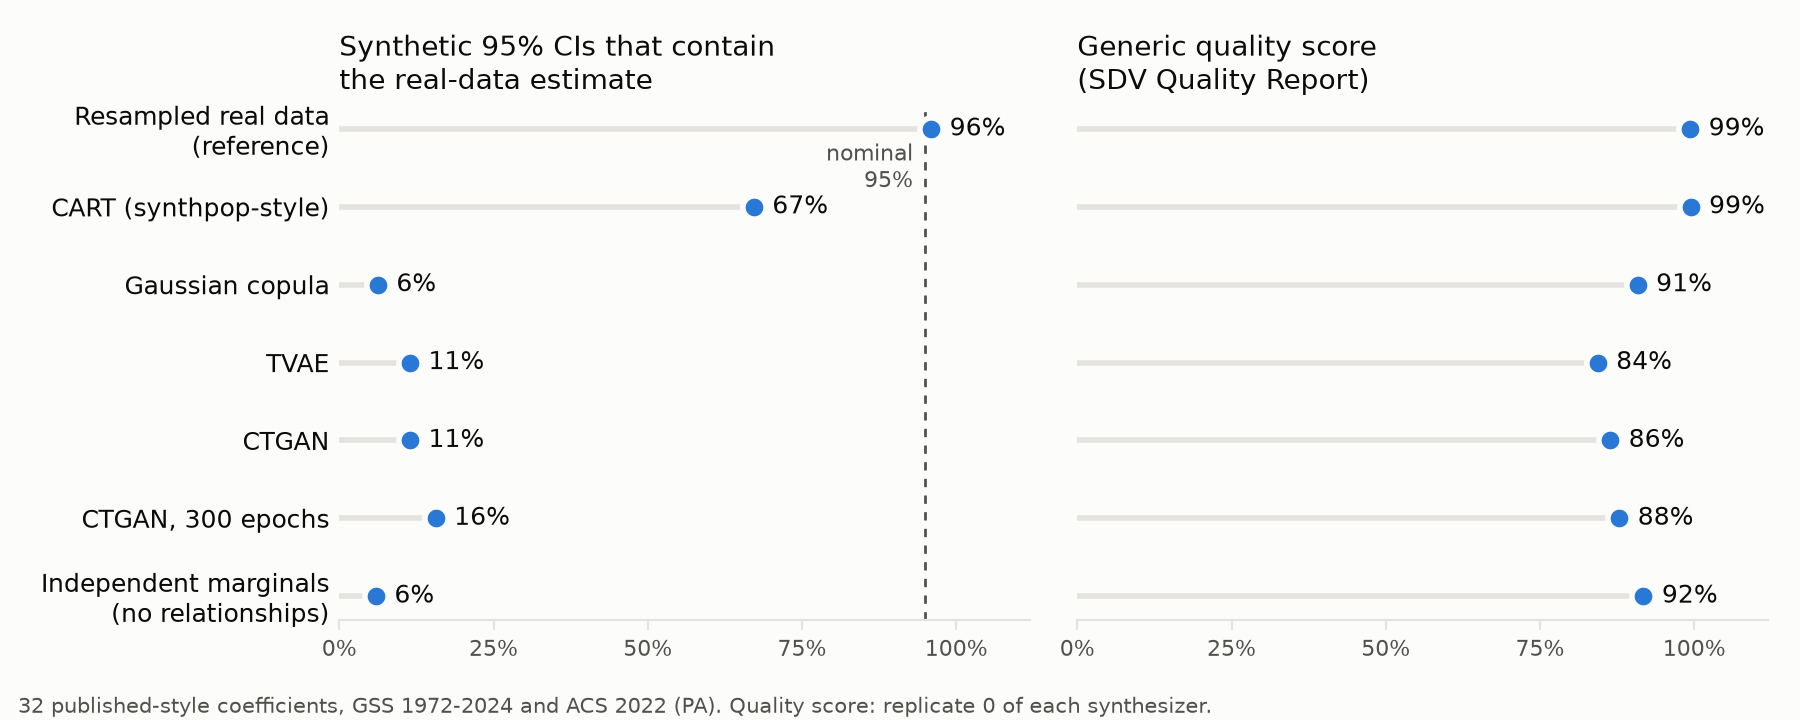
\includegraphics[width=\textwidth]{figure1.png}
\caption{Synthetic files that score 84--99\% on a generic quality report recover the real estimate for
as few as 6\% of published-style coefficients. A file with no relationships at all scores 92\%.}
\end{figure}

\section*{4. Contribution}
\begin{enumerate}
  \item \textbf{An analysis-level benchmark for synthetic social-science data.} Real public datasets, a
        battery of published-style estimands tagged by type, and reference and floor anchors, released as
        open code into which any synthesizer can be dropped.
  \item \textbf{A substantive warning.} Synthetic files certified by generic fidelity scores can reproduce
        significance stars while distorting effect sizes, especially for fixed-effects, nonlinear,
        interaction and subgroup estimates: exactly the quantities social scientists publish.
  \item \textbf{A practical protocol.} Releasers and users should report analysis-specific validity
        (coverage and CI overlap on a declared battery of estimands) alongside generic quality scores.
\end{enumerate}
This connects to the workshop's themes of validating AI-generated data, uncertainty quantification, and
replication.

\textbf{Plans for April.} Run R \texttt{synthpop} itself alongside our CART implementation; add
privacy-protected synthesizers (DP-CTGAN, smoothed CART) to map the privacy--validity frontier; add CPS
data and published replication archives analyzed with their authors' own models; incorporate survey
weights; and complete a preregistered full run with more replicates of the deep models.

\smallskip
\noindent\textit{Requested format:} lightning talk or talk; poster acceptable.
\quad\textit{Code and full reproduction:} \url{https://github.com/brandonyee-cs/synthrep}

\begingroup\small
\begin{thebibliography}{9}\setlength{\itemsep}{0pt}
\bibitem[Karr et~al.(2006)]{karr2006} Karr, A.\,F., Kohnen, C.\,N., Oganian, A., Reiter, J.\,P., \&
  Sanil, A.\,P. (2006). A framework for evaluating the utility of data altered to protect confidentiality.
  \emph{The American Statistician}, 60(3), 224--232.
\bibitem[Raab et~al.(2016)]{raab2016} Raab, G.\,M., Nowok, B., \& Dibben, C. (2016). Practical data
  synthesis for large samples. \emph{Journal of Privacy and Confidentiality}, 7(3), 67--97.
\bibitem[Reiter(2005)]{reiter2005} Reiter, J.\,P. (2005). Using CART to generate partially synthetic public
  use microdata. \emph{Journal of Official Statistics}, 21(3), 441--462.
\bibitem[Snoke et~al.(2018)]{snoke2018} Snoke, J., Raab, G.\,M., Nowok, B., Dibben, C., \& Slavkovi\'c, A.
  (2018). General and specific utility measures for synthetic data. \emph{JRSS Series A}, 181(3), 663--688.
\bibitem[Stevenson \& Wolfers(2009)]{stevenson2009} Stevenson, B., \& Wolfers, J. (2009). The paradox of
  declining female happiness. \emph{American Economic Journal: Economic Policy}, 1(2), 190--225.
\bibitem[Xu et~al.(2019)]{xu2019} Xu, L., Skoularidou, M., Cuesta-Infante, A., \& Veeramachaneni, K. (2019).
  Modeling tabular data using conditional GAN. \emph{NeurIPS}.
\end{thebibliography}
\endgroup
\end{document}
